\section{Feature Interaction}
\label{sec:feature_interac}
The interaction between features must also be considered: for instance, even if
a feature is seemingly unrelated to the target variable, when seen in
combination with other features, patterns may emerge. In order to study the
interaction among features, we created movie scatter plots where dot colors are
set according to movie performance groups, and axes represent features'
normalized values.

Specifically, Figure~\ref{fig:interaction} shows the formation of colored
clusters. The colors encode team's performance, which indicates that certain
combination of features can be used to help identifying team's performance. To
take advantage of this phenomena, we also included the product of every feature
pair as new features. There are dozens of possible pairs such that analysing
every pair individually is not practical. Machine Learning techniques are
employed to automatically identify pairs that add the most relevant
information. Figure~\ref{fig:interaction} presents some of the relevant pairs
for illustrative purposes.

There are two ways to calculate feature interaction: normalizing the features
to the [0--1] interval (using a simple linear interpolation) and then
calculating their product, or doing the same in reverse order. From
experimental evaluation, both methods produce similar results, but normalizing
before calculating the product performs slighting better. We assume this
happens because multiplying variables of the same magnitude mimics better the
way in which variables interact.

\begin{figure}[t]\begin{center}
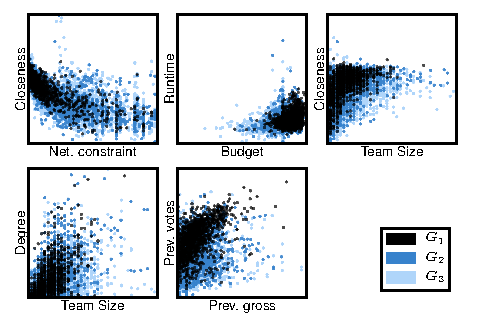
\includegraphics[width=\columnwidth]{../../images/feature_interaction.pdf}
\caption{\label{fig:interaction}Joint scatter plot of movies per features. The
shade of a point represents its performance group. Dark clusters form 
in the graph, meaning iteration between features should be considered.}
\end{center}\end{figure}
